\section{Visualization}

Visualization techniques are used to understand the data better and also used to more clearly bring out patterns and relationships in the dataset. Further, appropriate visualizations serve as a medium of choosing the correct data mining tasks on the dataset. Additionally, the visualizations help gauge the difficulties one may face while working with the dataset. 
The chosen dataset is highly dimensional and has a lot of points (rows) in the dataset. This makes the task of visualization harder as it is difficult to fit approximately 400,000 points on a single graph without cluttering. Moreover, the high dimensionality of the dataset makes it harder to visualize the data in a 2D or 3D graph which accurately represents the dataset. Dimensionality reduction algorithms like PCA and LDA do not work well on this dataset because half the dataset is categorical in nature and condensing the numerical census data into lesser features does not make sense. 
To overcome these issues, the dataset was randomly sampled to make some of the plots. This solves the issue of having too many points. To fix the issue of high dimensionality, only a few features were taken at a time and plotted to get specific and meaningful graphs regarding the selected features. This process is repeated for many significant features to get a basic understanding of the dataset.

\begin{figure}[h]
\centerline{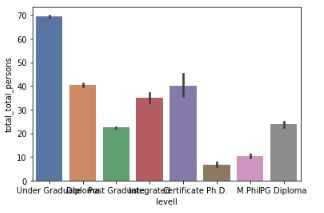
\includegraphics{figures/degrees.jpg}}
\caption{Distribution of students in various degrees}
\label{deg}
\end{figure}

Fig.~\ref{deg} depicts the distribution of the students in different higher education degrees. It is clearly seen that Under graduate degrees are very common and Ph.D degrees are very less in India. This may be due to most Indian students preferring to do their post graduations abroad. 

\begin{figure}[h]
\centerline{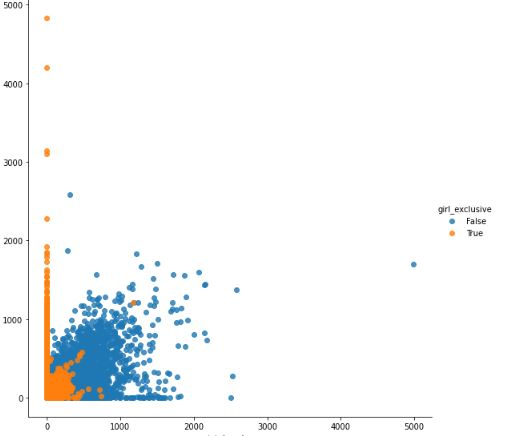
\includegraphics[scale=0.6]{figures/girls_general.jpg}}
\caption{Distribution girls in general category vs muslim girls}
\label{girls}
\end{figure}

In Fig.~\ref{girls}, the number of general community females are plotted against the number of muslim community females and are divided by female exclusive colleges, it is clearly seen that the muslim community prefers to enroll more in female-only colleges as compared to the general category.

Fig.~\ref{study_years} shows the comparison of number of years of study of general caste vs backward castes. A general tread of 1-2 years of study can be seen among backward caste people which shows that they prefer smaller undergraduate degrees and do not often pursue post graduate studies.

\begin{figure}[h]
\centerline{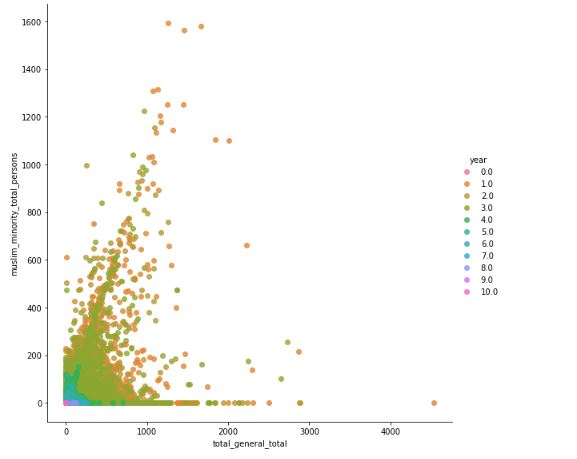
\includegraphics[scale=0.6]{figures/years_study.jpg}}
\caption{Comparison of number of years of study in backward castes vs general caste}
\label{study_years}
\end{figure}

\begin{figure}[h]
\centerline{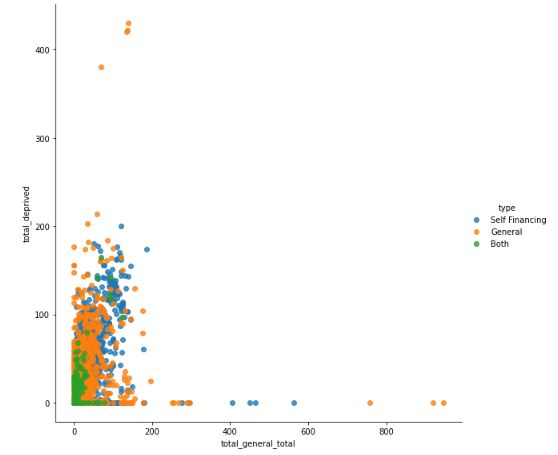
\includegraphics[scale=0.6]{figures/hyd.jpg}}
\caption{Distribution of degrees in Hyderabad based on financial type}
\label{hyd}
\end{figure}

It is observed from Fig.~\ref{hyd} that people in metro cities like Hyderabad prefer self-financing degrees whereas the opposite trend is observed throughout the rest of the country where self-financing is least preferred.